\documentclass[12pt,a4paper]{article}
\usepackage[utf8]{inputenc}
\usepackage[russian]{babel}
\usepackage{amsmath}
\usepackage{amsfonts}
\usepackage{amssymb}
\usepackage{graphics}
\usepackage[pdftex]{graphicx}
\usepackage{lscape}
\usepackage{listings}
\lstset{
breaklines=true, % Перенос длинных строк
basicstyle=\ttfamily\footnotesize, % Шрифт для отображения кода
frame=tblr % draw a frame at all sides of the code block
tabsize=2, % tab space width
showstringspaces=false, % don't mark spaces in strings
% Настройка отображения номеров строк
numbers=left, % Слева отображаются номера строк
stepnumber=1, % Каждую строку нумеровать
numbersep=5pt, % Отступ от кода
}
\renewcommand{\lstlistingname}{Листинг} 
\author{Анастасия Тарасова}
\title{Отчет по лабораторной работе №1 :\\ \LaTeX{}, Git, GPG}
\begin{document}
\maketitle
\section{Система верстки \TeX{} и расширения \LaTeX{}}
\subsection{Цель работы}
Освоить систему верстки \TeX{} и сделать отчет.
\subsection{Ход работы}
В ходе работы был создан файл с расширением .tex, в котором содержатся команды текстовой разметки.
\subsubsection{Компиляция в командной строке}
Исходными данными для \LaTeX{} является обычный текстовый файл с расширением .tex. Его можно создать в текстовом редакторе. Существуют текстовые редакторы общего назначения с поддержкой \LaTeX{} (Emacs, vim, geany, Eclipse, Notepad++, TextMate, Sublime Text и т.д.), специализированные текстовые LaTeX-редакторы (TeXstudio, Texmaker, gummi, Kile, TexShop, TeXnicCenter, WinEdt и т.д.), визуальные редакторы (LyX, TeXmacs и BaKoMa TeX Word).  Tex-файл содержит текст документа вместе с командами, указывающими \LaTeX{}, каким образом верстать текст.
Создание pdf-документа по входному файлу выполняется следующим образом:

\begin{itemize}
\item В командной строке необходимо выполнить команду

\verb+latex <имя входного файла без расширения>+

Команда преобразует входной файл в в файл формата dvi (Device Independent), пригодный к распечатке.
В настоящее время файлы формата dvi используются для предпросмотра итогового документа.
Файл dvi можно просмотреть при помощи утилиты Yap, распространяемой вместе с дистрибутивом MikTeX.
\item xdvi одна из программ DVI-драйверов, позволяющих отображать данные в формате
DVI в X Window системах

\verb+xdvi report1.dvi+

Результат показан на рисунке 1.
\begin{figure}[h!]
\centering
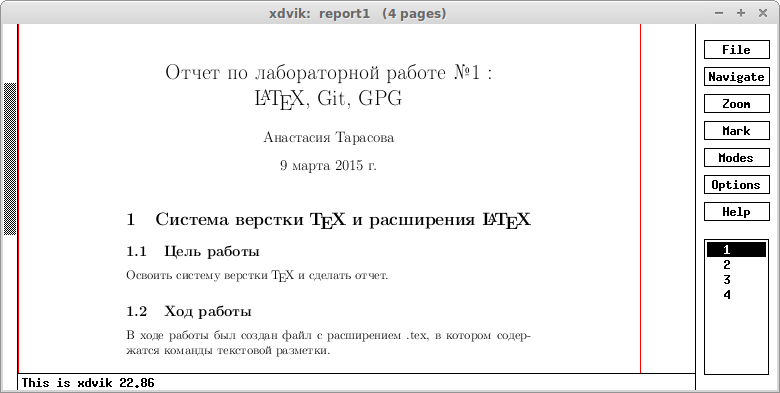
\includegraphics[scale=0.5]{res/xdvi}
\caption{Заппуск xdvi}
\end{figure}

\item
\verb+pdflatex report1.tex+

Команда создает итоговый pdf-документ.
\end{itemize}

\subsubsection{Оболочка TexMaker}
TexMaker - текстовый редактор, работающий с языком разметки LaTeX. TexMaker позволяет работать с фишками профессионального оформления. Внешний вид редактора представлен на рисунке 1. В редакторе TexMaker имеется возможность быстрой сборки и быстрого старта. Чтобы задать преамбулу документа, можно использовать помошника "Быстрый старт" (Меню "Помошник").Этот диалог позволяет задать главные особенности Вашего документа (класс, размер бумаги, кодировку...).
\begin{figure}[h!]
\centering
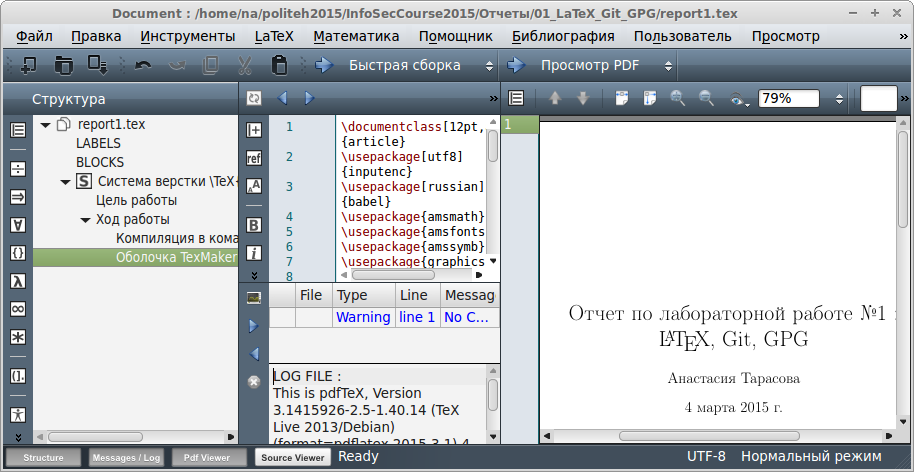
\includegraphics[scale=0.5]{res/texmaker}
\caption{Редактор TexMaker}
\end{figure}
\subsubsection{Классы документов}
В самом начале файла указывается класс документа, который задается командой\\\\
\verb+\documentclass[опции]{класс}+
\\\\Здесь класс определяет тип создаваемого документа. Опции изменяют поведение класса.\\\\
\verb+\documentclass[12pt,a4paper]{article}+ 
\\\\Эта строчка заставляет \LaTeX{} применить следующие правила для документа:

\begin{itemize}
\item[] Набирать документ как статью
\item[] Базовый размер шрифта - 12
\item[] Форматирование для печати на бумаге формата А4
\end{itemize}

\subsubsection{Подключаемые пакеты}
В процессе написание документа в некоторых областях базовый \LaTeX{} не сможет решить некоторые проблемы. В подключаемых пакетах можно указать особые настройки.
\\\\
\verb+\usepackage{lscape}+
\\\\
Данный пакет меняет положение страницы на ландшафтное

\subsubsection{Верстка формул}
\begin{itemize}
\item Степени и индексы

$a^2+b^2=c^2;$

$a_2-b_2=c_2;$

$a_3^2+b_3^2=c_3^2;$
\item Дроби

$\frac{a_3^2+b_3^2}{c_3^2};$

\item Скобки

$f\{x,y\}=(x^2+y^2)^2 ;$

$\lceil X \rceil, \lfloor Y \rfloor, \langle Z \rangle;$

\item Корни, интегралы и дифференциалы

$\sqrt[3]{x+y};$

$\int_{0}^{3} f(x) dx ;$

$\iint_{x^2 + y^2 = 1} f(x, y) dx dy   ;$

$\iiint_{x^2 + y^2 + z^2 = 1} f(x, y, z) dx dy dz;$

$dz = \frac{\partial z}{\partial x} dx + \frac{\partial z}{\partial y} dy ;$
\end{itemize}

\subsection{Выводы}
\LaTeX{} – это система набора текста, основанная на специальном скриптовом языке программирования. \LaTeX{} уже давно является стандартом де-факто при наборе научных статей, курсовых и дипломных работ, технических спецификаций, учебников и т. д. Главным преимуществом \LaTeX{} является абсолютно одинаковый внешний вид готовых страниц во всех операционных системах и непревзойденное до сих пор качество полиграфических текстов и математических формул. Кроме этого, скриптовый язык латеха – это универсальный язык для обмена формулами.

\newpage
\section{Система контроля версий Git}

\subsection{Цель работы}
Научиться работать с системой Git.
\subsection{Ход работы}
\begin{itemize}
\item Получить содержимое репозитория

\verb+ git clone https://github.com/AnastasiyaTarasova/InfoSecCourse2015.git+

\item Работа с ветками

\verb+git checkout -b laba1+ -создвем ветку

\verb+git push origin laba1+ - публикуем ее

\verb+git branch+ - смотрим список веток

\verb+git checkout master+ - переключаемся на ветку master

\item Зафиксировать изменения в локальном и центральном репозитории

\verb+git commit -a -m "file changed"+ 

\verb+git push+ 

\item Вытянуть изменения

\verb+git pull+

\end{itemize}

\subsection{Выводы}
GitHub это социальный репозиторий для проектов с открытым исходным кодом, использующих Git для контроля версий исходного кода. Главная задача GitHub - сделать процесс разработки простым и увлекательным, в особенности когда над проектом одновременно работает несколько человек. Использование GitHub также позволяет научиться многим вещам. Базовым кирпичиком git репозитория является коммит (commit). Код со временем меняется, но если вы делаете коммиты, то к любому из них можно вернуться, отмотав время назад с помощью git.
\newpage
\section{Cоздание электронных цифровых подписей c PGP}

\subsection{Цель работы}
Научиться создавать сертификаты, шифровать файлы и ставить ЭЦП.
\subsection{Ход работы}

\subsubsection{Знакомство с пакетом Kleopatra}
Kleopatra это графический интерфейс к GnuPG и предназначенных для работы под
окружением KDE и портированный на MS Windows (доступные в составе пакета Gpg4win).

При помощи мастера, графический интерфейс позволяет создать сертификат. Его текстовый вид представлен в листинге 1.

\lstinputlisting[language={},caption={Сертификат в формате asc (ASCII Armored file)}]{res/8800CC12EA6C611230C3B6EAA0F30A9FC02028FC.asc}
Подпись документа можно сделать используя закрытый ключ. Цифровая подпись сохраняется в отдельный файл с расширением sig. Если зашифровать файл \textit{report1.pdf}, то подпись будет сохранена в файле \textit{report1.pdf.sig} (см. рис. 5).

Программа позволяет импортировать чужие сертификаты, и проверять подписи. На рисунке
6 показан итог импорта чужого файла.


\begin{figure}[h!]
\centering
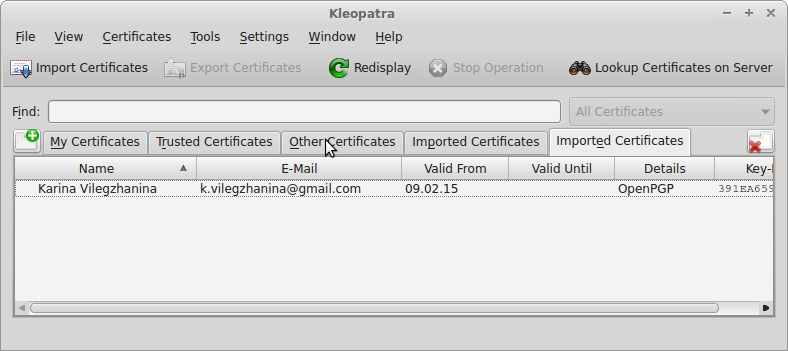
\includegraphics[scale=0.5]{res/karina}
\caption{Импорт чужого ключа в Kleopatra}
\end{figure}
\subsubsection{Использование gpg через интерфейс командной строки}

Результат, полученный при помощи Kleopatra легко повторить используя терминал. Генерация ключа происходит в диалоговом режиме после ввода команды
\begin{verbatim}gpg --gen-key
\end{verbatim}
В процессе работы, мастер создания ключа запросит следующую информацию:
\begin{itemize}
\item{Тип ключа (по умолчанию это DSA и ElGamal).}
\item{Размер ключа (с DSA/ElGamal ключами не использую длину больше чем 2048).}
\item{"срок годности" ключа.}
\item{Информацию о пользователе (имя, электронный адрес).}
\item{Пароль для ключа (если нужен).}
\end{itemize}
В процессе генерации ключа, GnuPG использует энтропию. Для способствования её сбору рекомендуется активно двигать мышкой или запустить mp3 в фоновом режиме.
Просмотреть доступные в системе ключи позволяет команда
\begin{verbatim}gpg --list-keys
\end{verbatim}
Её вывод показан ниже.
\begin{figure}[h!]
\centering
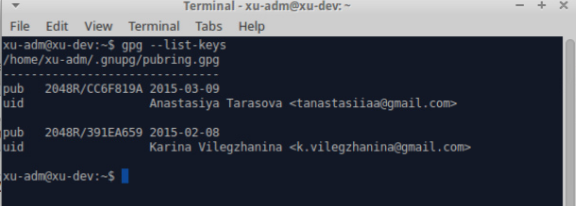
\includegraphics[scale=0.8]{res/gpgterminal}
\caption{Список ключей в системе.}
\end{figure}
Для экспорта можно использовать команду (ключ определяется по электронному адресу)
\begin{verbatim}gpg --armor --output john.asc --export john@mail.ru
\end{verbatim}
Для импорта используется
\begin{verbatim}gpg --import tomas.asc
\end{verbatim}
\subsection{Выводы}
GnuPG шифрует сообщения, используя асимметричные пары ключей, генерируемые пользователями GnuPG. Открытыми ключами можно обмениваться с другими пользователями различными путями, в том числе и через интернет с помощью серверов ключей. Также GnuPG позволяет добавлять криптографическую цифровую подпись к сообщению, при этом целостность и отправитель сообщения могут быть проверены. 
\end{document}
